\SetPicSubDir{ch-Univariate}
\SetExpSubDir{ch-Univariate}

\chapter{AIS-based Trajectory Prediction Model}
\label{ch:univariate}
\vspace{2em}

\section{Preliminaries}
In the data science pipeline, the next stage after data exploration and visualization is data preparation and transformation \cite{geron2017handson}. This chapter attempts to predict the future movements of the vessel using a prediction model. We will first prepare AIS datasets in a usable form and then proceed with the development of the model. In dealing with movement data, \cite{liraz2018ships} and \cite{graser2020open} provides a description of the process and tools that we use in the following sub-section.

\subsection{Defining Ship Track}
Recalled from the Data Description part in Chapter \ref{ch:eda}, AIS data consist of dynamic and static records. Dynamic records include a timestamp, MMSI, longitude, latitude, and other information. We use a data object called POINT implemented by Shapely library to transform longitude and latitude into a single coordinate object for easier object manipulation. We will use the term coordinate and POINT interchangeably for the rest of this chapter, and by that we are referring to longitude and latitude as well. The ship track is defined as a consecutive POINTS of the ship of various lengths. The behavior of tracks vary from one another; one track might be a continuous sailing within a short period, another might include months of sailing with multiple anchoring points \cite{liraz2018ships}. We observe that many tracks consist of few POINTS. Shorter tracks less than 100 meters or 30 POINTS are excluded from the list to ensure our tracks carry enough information for the neural network to learn the pattern. A track also would be split into two in the event of the time interval between consecutive records is more than 15 minutes. The 15 minutes tress-hold is derived from our finding that time interval between AIS consecutive records makes up from 0.96 seconds up to 6 days with 75\% of the records account for 16 minutes of the time interval. The process of collecting, filtering, and splitting tracks from the unstructured AIS dataset is done using ``movingpandas'' library. Movingpandas \cite{graser2020open} and Shapely are dedicated python package designed for spatial data analysis and manipulation.

\subsection{Handling Missing and Erroneous Data}
We summarised missing and erroneous value by the AIS field in the previous chapter and recalled that while longitude, latitude and MMSI do not have missing value, they both suffer from erroneous value by 3\% and 5\% respectively. In dealing with erroneous data, we filtered out those records with invalid value criteria as mentioned in Table \ref{tab:table5} of Chapter \ref{ch:eda}. We also limit our data observation into the Singapore Straits region as an additional way to filter out the erroneous coordinates.

Spline and Linear interpolation are the two techniques we used to fill missing data. Interpolation is as an approach of constructing new variable values given a discrete set of its intermediate values. We use interpolation in response to the fact that the AIS time series is not evenly sampled and hence the data is considered missing at a certain point of time. According to \cite{beveridge1992least} in \cite{lepot2017interpolation}, a useful interpolation technique should meet four criteria: (i) not a lot of data required to fill the missing values; (ii) estimation of parameters of the model are permitted; (iii) efficient data computation; (iv) the technique should applicable to stationary and non-stationary. 

The spline is one of the interpolation technique with smoothing parameters. Smoothing is useful when there are many outliers in a dataset like AIS records so that the interpolated curve would focus on finding the main values. Outliers are a problem for the machine learning model especially if the numbers are high as the model would learn from false information and would output false inference. Linear interpolation is another interpolation that tries to fit a set of values using linear polynomial to construct new data. Spline and Linear interpolation are supported by Scipy, a python-based ecosystem for scientific computation. There are several Spline and Linear methods in Scipy depending on the problem, we use LSQ Univariate Spline for its one-dimensional spline interpolation with explicit internal \emph{knots} and Interp1D for Linear interpolation. We observe that the Linear technique is less sensitive towards the outlier coordinate as compared to Spline. However, the Linear technique does not overly smooth-off the curve as the Spline does which is somewhat closer to the actual curve. Figure \ref{fig:interp} shows the 3 trajectories as a comparison.

\begin{figure}[t!]
    \centering
    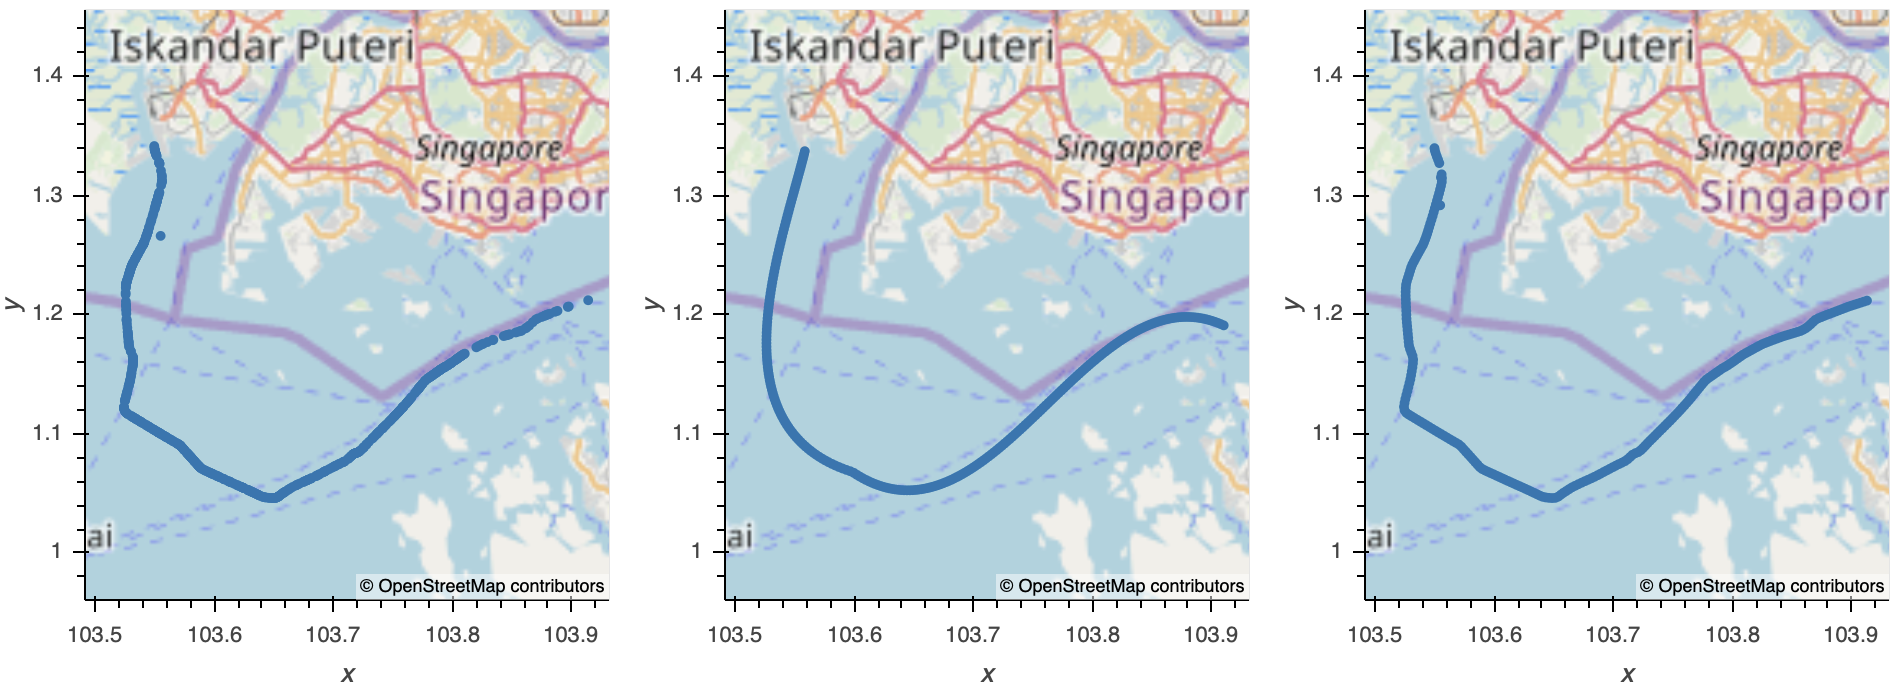
\includegraphics[width=15cm]{pic/ch-Univariate/interpolations.png}
    \caption{Trajectory interpolation of 2 methods. Left: Normal. Center: Spline. Right: Linear. Notice the single noise in the Left and Right}
    \label{fig:interp}
\end{figure}

\section{Methodology}

\begin{figure}[t!]
    \centering
    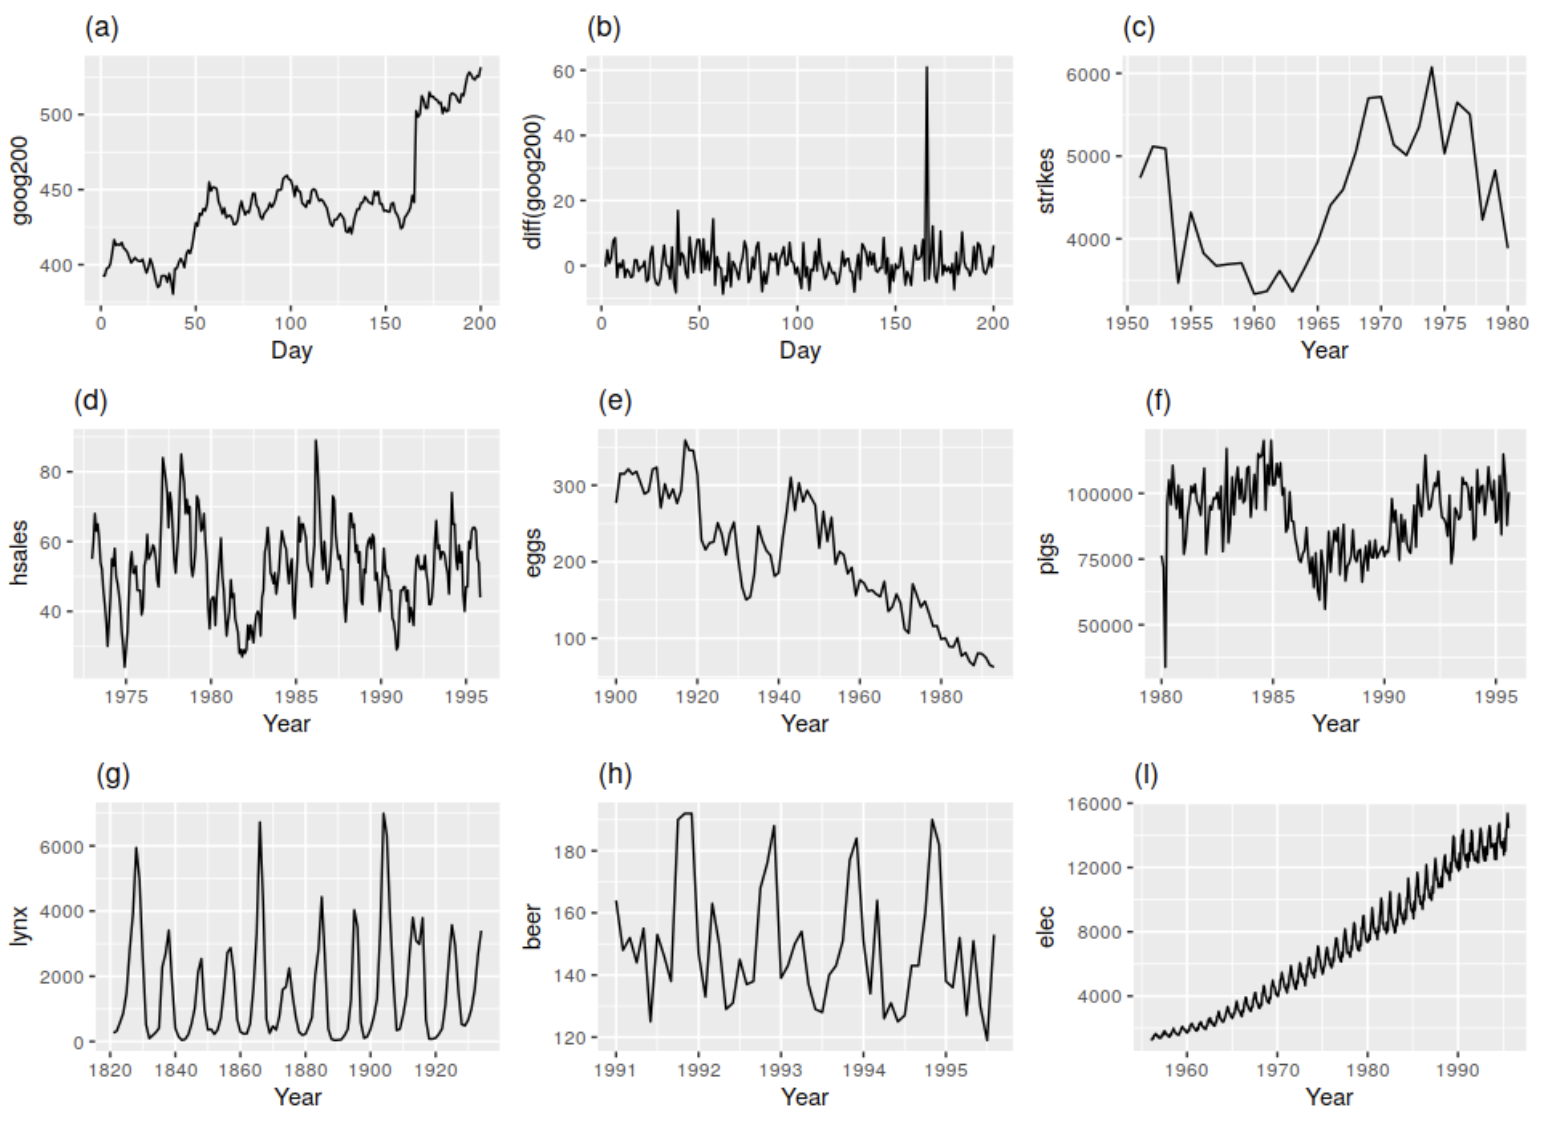
\includegraphics[width=15cm]{pic/ch-Univariate/stationary.png}
    \caption{Which of these series are stationary? (a) Google stock price for 200 consecutive days; (b) Daily change in the Google stock price for 200 consecutive days; (c) Annual number of strikes in the US; (d) Monthly sales of new one-family houses sold in the US; (e) Annual price of a dozen eggs in the US (constant dollars); (f) Monthly total of pigs slaughtered in Victoria, Australia; (g) Annual total of lynx trapped in the McKenzie River district of north-west Canada; (h) Monthly Australian beer production; (i) Monthly Australian electricity production. (Figure taken from Forecasting: Principles and Practice by Rob J Hyndman)}
    \label{fig:stationary}
\end{figure}

\begin{figure}[t!]
    \centering
    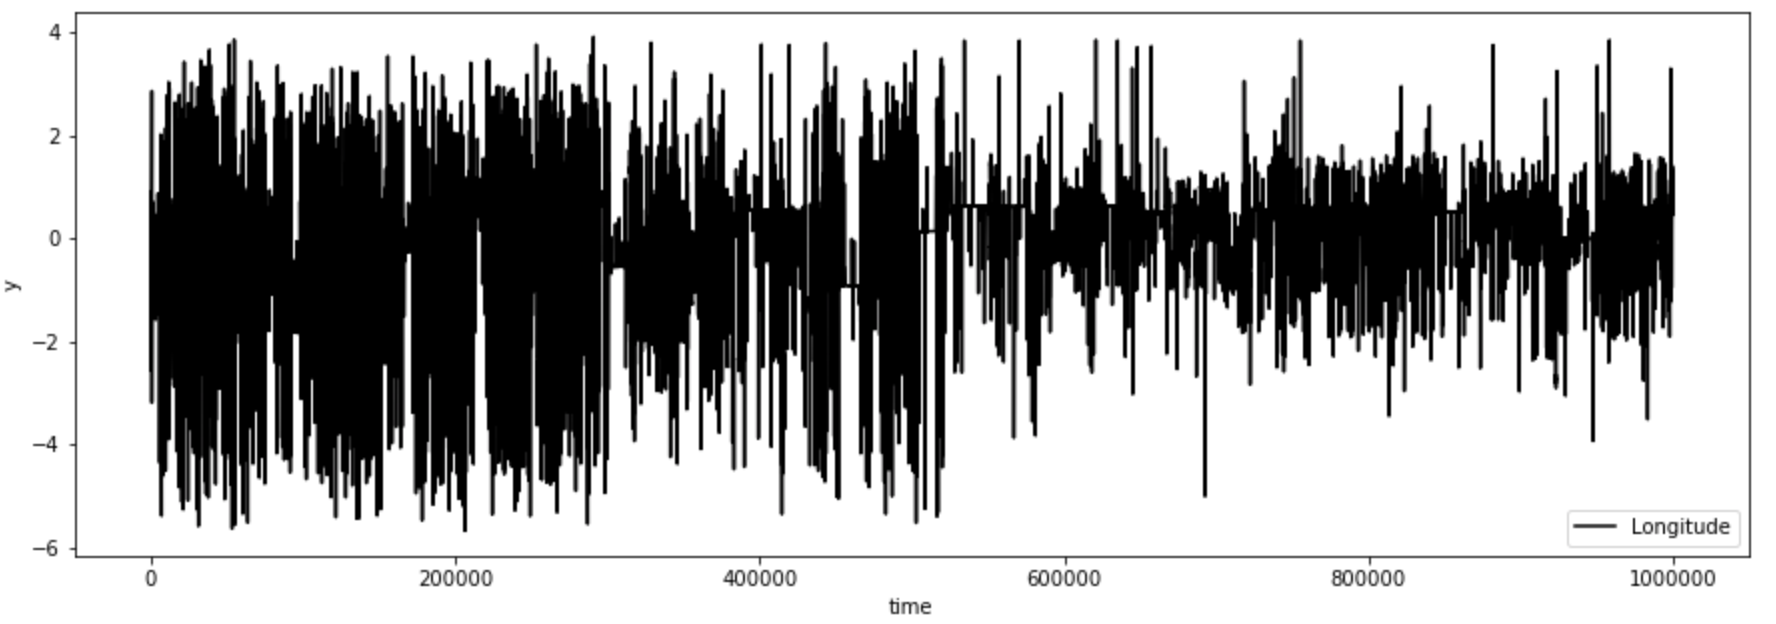
\includegraphics[width=14cm]{pic/ch-Univariate/longitude.png}
    \caption{Longitude AIS time series data for 1 month}
    \label{fig:longitude}
\end{figure}

The research question we need to answer in this project is, how can we develop a model to best predict the future movement of the vessel given their historic navigation information. To answer this question, we use the AIS time series data collected in Singapore Straits during December 2019 period. There are two most common approach for predicting time series models that can be applied to our problem; statistical and machine learning (including artificial neural network) approach. A statistical approach for time series prediction has been used in application such as stock market forecasting even before machine learning become popular. The objective of machine learning is the same as that of statistical ones. They both aim at improving prediction accuracy by minimizing some loss function, typically \emph{mean absolute error} or \emph{mean square error} \cite{makridakis2018statistical}. The difference between the two lies in the fact that the statistical method assumes the data to be stationary and the algorithm is linear while the machine learning model assumes none of them. A stationary time series is one whose statistical properties such as mean, variance, auto-correlation do not change over time. Thus, time series with trend and seasonality are not stationary \cite{hyndman2018forecasting}. Figure \ref{fig:stationary} shows some examples of stationary data over a different dataset. Figure \ref{fig:stationary}.b and \ref{fig:stationary}.g are the only stationery series while the rest are not. 

Although a study by Makridakis \emph{et al.} suggest that some statistical methods outperform machine learning and neural network model on M3 competition dataset, we decide to use machine learning models in the experiment of this chapter one reason; AIS time series data as shown in Figure \ref{fig:longitude} is not stationary. The data consist of many vessel types (e.g. passenger, cargo, tanker, etc) with different navigation status across a different period of voyage. That itself ruled out the data to be stationary. We will experiment using a simple machine learning model for baseline; a Linear Regression. The next model to develop an attempt to improve the accuracy of this baseline result.

With the machine learning model, the problem of predicting future vessel trajectory can be achieved with either regression (predicting value) or classification task (predicting class), depending on the output representation. The classification approach for movement data typically starts with trajectory clustering and proceeds with assigning a new trajectory to the closest cluster to decide where the next vessel's position is. The regression approach, on the other hand, predicts the actual value of the vessel's next position by using a set of input features and target labels. We believe that the classification approach is worth exploring but due to our time limitation we will focus on using the regression task for this thesis.

As we have narrowed down to use machine learning and neural network model, it is important to understand that the two models accept different input representations. Input representation is the way we transform the dataset into a usable form that is understandable by the model. The earlier section of \ref{ch:univariate} has pre-processed AIS data into a collection of tracks grouped by track id. The pre-processed dataset has 2584 unique MMSI and 10812 tracks over the course of 1 month AIS data. As seen in figure 4.4, the time series data consist of a two-time column, one in datetime format, another in an integer format. It also consists of 2 IDs to identify a coordinate, one is MMSI ID, another is Track ID where a single MMSI ID may consist of some Track ID as happened in a long voyage of the ship with the large time interval gaps being split into multiple tracks. Lastly the data is sorted by track id in increasing order. This will become our base dataset for the machine learning model.

\begin{figure}[t!]
\centering
\begin{subfigure}[b]{.45\textwidth}
  \centering
  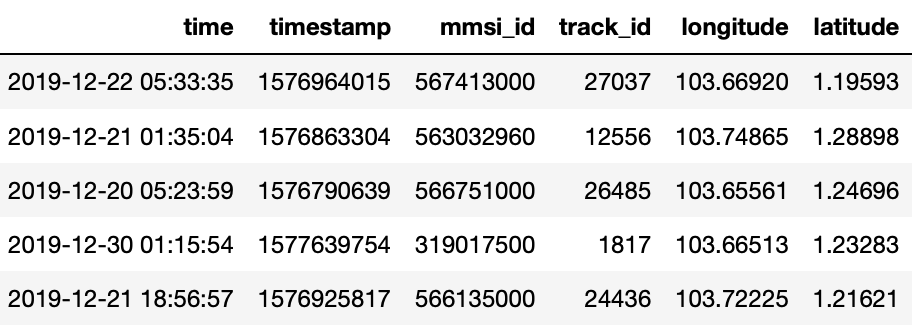
\includegraphics[width=1\linewidth]{pic/ch-Univariate/dataset_random.png}
  \caption{Before sorted by track id}
  \label{fig:dataset_sub1}
\end{subfigure}
%
\begin{subfigure}[b]{.45\textwidth}
  \centering
  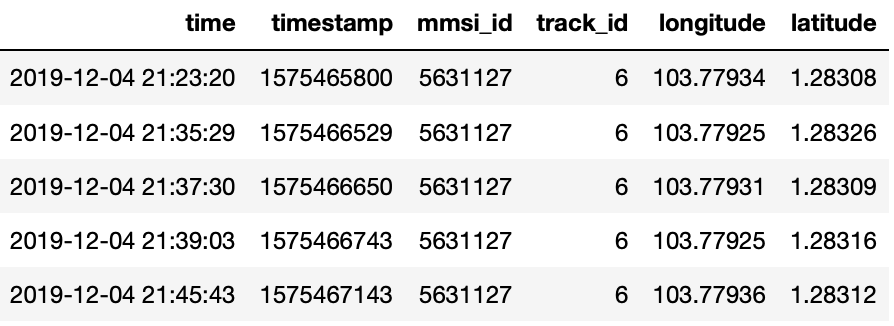
\includegraphics[width=1\linewidth]{pic/ch-Univariate/dataset_head.png}
  \caption{After sorted by track id}
  \label{fig:dataset_sub2}
\end{subfigure}
\caption{Pre-preocessed AIS dataset}
\label{fig:dataset}
\end{figure}

Time series data has a property called sequence for their input in addition to samples and features. The sequence is a consecutive observation of input from the time step t backward. We define the number of observation sequences as the window size. Time series data also has a sequence of prediction from the time step t forwards. We define the number of prediction sequence as response size. For response size of 1, we called it a single-step prediction and for response size of more than 1, we called it a multi-step prediction. It is also possible for time series data to have multiple variables prediction instead of just one, hence called multivariable prediction. The problem we want to solve is characterized as a multi-step and multivariable prediction. If we look at AIS data in Figure \ref{fig:dataset}, our time series data is not evenly sampled or irregular. There are two ways to handle the irregularity of time series, first is to downsample or oversample the data with a specified period (e.g., minute, hour, day) using interpolation as we discussed in Section 4.1.3. Downsampling data would result in generating more data while oversampling data on the contrary is reducing the number of data. Secondly, it is to keep the irregular time series unaltered and let the prediction model learn the time dependency. This can be achieved by inserting a time difference between timestamp t+1 and t as a new input feature in addition to longitude and latitude.

\subsection{Machine Learning Input Representation}

\begin{figure}[t!]
    \centering
    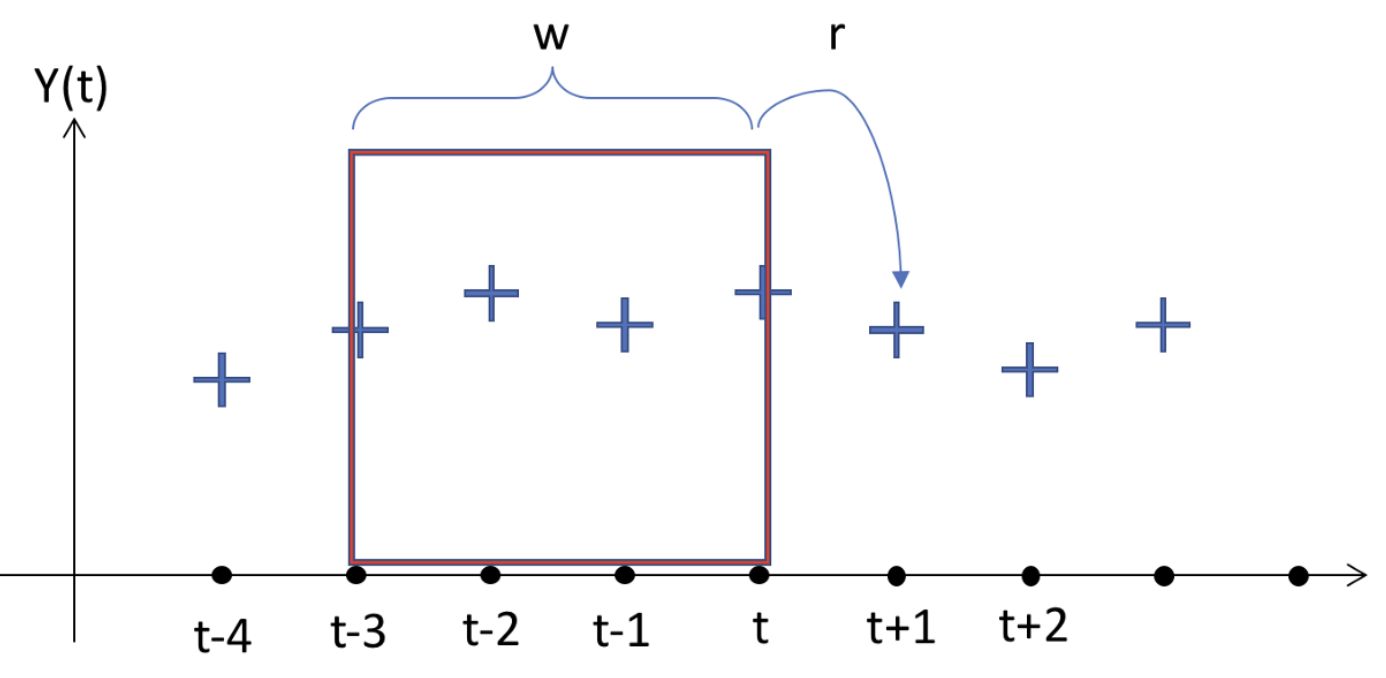
\includegraphics[width=12cm]{pic/ch-Univariate/sliding.png}
    \caption{Sliding window method to transform time series into sequential supervised learning input. Figure taken from Pablo Ruiz}
    \label{fig:sliding}
\end{figure}

Machine Learning model accepts 2-dimensional input and 1-dimensional output. The input is the number of samples of several features while the output is the number of samples of one target variable. The two-dimension input and one dimension output are often called supervised learning problems. It is not the nature of the machine learning model to work with time-series data that involves window size and response size of more than 1. In the need of solving the time series problem with the machine learning model, we need to phrase it as a sequential supervised learning problem by using the sliding window method. The \emph{sequential supervised learning} problem can be formulated as follows. Let $\{(\Vec{x}_i, \Vec{y}_i)\}_{i=1}^{N}$ be a set of \emph{N} training examples. Each example is a pair of sequence $(\Vec{x}_i, \Vec{y}_i)$, where $\Vec{x}_i = \langle \Vec{x}_{i,1}, \Vec{x}_{i,2}, \Vec{x}_{i,3}, ..., \Vec{x}_{i,T_w} \rangle$ and $\Vec{y}_i = \langle \Vec{y}_{i,1}, \Vec{y}_{i,2}, \Vec{y}_{i,3}, ..., \Vec{y}_{i,T_r} \rangle$ where \emph{w} and \emph{r} represents windows size and response size. The goal is to construct a classifier \emph{h} that can correctly predict a new label sequence $\Vec{y} = \emph{h}(\Vec{x})$ given an input sequence of \Vec{x} \cite{dietterich2002machine}. The sliding window method is illustrated in Figure \ref{fig:sliding} where the window size is 4 and the response size is 1. We transform each sequence of time series data from the 3-dimensional shape into 2 dimensional one. For the first sequence, the sliding window observes features from time step t to t-3 and indicates the target variable at t+1 as the output. The result is a metric of shape 4$\times$3. Next the metrics need to be flattened into a shape of 1$\times$12 allowing each observation at any time-step t become a feature of its own. The sliding process continues from time-step t+1 to t-2, t+2 to t-1 and so on until all dataset has been covered. Our final dataset transformation is presented in Figure \ref{fig:after_transformed} with the original dataset in Figure \ref{fig:original}. The blue box and red box in Figure \ref{fig:original} represent a set of input and output for a single observation. Each column values are flattened and become new features in Figure \ref{fig:after_transformed}. The last input feature delta-t(5) is added to indicate that the output is taken from time-step 5 and hopefully the model could learn the pattern. The output Y in Figure \ref{fig:after_transformed} comes from the red box of either longitude or latitude feature.

\begin{figure}[t!]
\centering
\begin{subfigure}[b]{.30\textwidth}
  \centering
  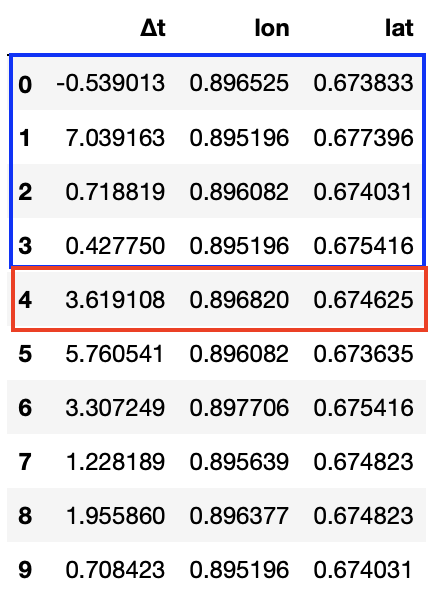
\includegraphics[width=1\linewidth]{pic/ch-Univariate/original.png}
  \caption{The original dataset before feature transformation has 3 features}
  \label{fig:original}
\end{subfigure}
%
\begin{subfigure}[b]{.85\textwidth}
  \centering
  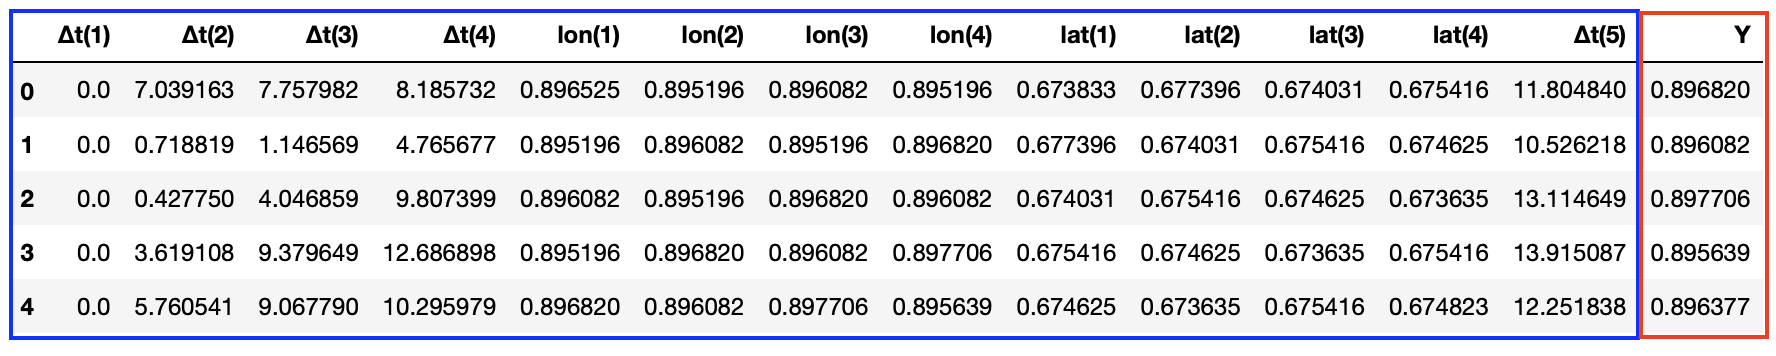
\includegraphics[width=1\linewidth]{pic/ch-Univariate/transformed.png}
  \caption{The transformed dataset has total 13 input features and 1 output target out of window size 4 and response size 1}
  \label{fig:after_transformed}
\end{subfigure}
\caption{AIS dataset transformation}
\label{fig:transformed}
\end{figure}

\subsection{Neural Network Input Representation}
Our neural network model consists of a stack of Long Short Term Memory (LSTM) and Dense layer. The input-output of the LSTM and Dense layer differ slightly as compared to the machine learning one. To work with our mentioned model, we need to transform the input and target dataset into a sequence of coordinate using a defined window size N and response size R. This can be achieved by shaping the input dataset in 3-dimension where the first dimension represents the batch size, the second dimension represents the window size N from time step t to t-N-1, and the third dimension represents the number of feature in the input sequence, which in our case 2 features for longitude and latitude. The target dataset would have a shape of 2-dimension where the first dimension represents the response size R from timestep t+1 to t+R, and the second dimension represents the number of features in the target sequence, which also happens to be longitude and latitude. The process of creating an input sequence is illustrated in Figure 4.6a using window size N of 4 and response size R of 1. The total new input size is M-N-R+1 given the number of datasets is M.

\subsection{Loss Function and Evaluation Metric}
Loss Function and Evaluation Metric often share the same definition; they both are a method of evaluating model performance quantitatively, but they serve a different purpose. The loss function is used to optimize the model during training while the evaluation metric is used to measure the performance of the model. The former is a reference for an optimization algorithm to help reduce the error, while the other one has no relation to the optimization algorithm. In the regression problem, the function used for loss function can also be used as an evaluation metric. The most commonly used loss function for regression are \emph{Mean Absolute Error} and \emph{Root Mean Squared Error}, and we add more evaluation metric called \emph{Mean Absolute Percentage Error}.

\begin{itemize}
    \item Mean Absolute Error (MAE) or often called L1 loss, is measured as the average sum of the absolute difference between prediction and the actual value. Since MAE take the absolute difference as the loss, it is considered robust towards outlier and hence suitable for a dataset with many outlier or noise. Mathematically calculated using the following formula: MAE = $\frac{1}{n}\Sigma_{i=1}^{n}{|y_i - \hat{y_i}|}$.
    \item Root Mean Squared Error (RMSE), is measured as the square root of the average sum of the squared difference between prediction and the actual value. If the difference between prediction and the actual value is large, perhaps due to the outlier, the root square of it would be larger as compared to the absolute error approach. Therefore RMSE is preferred if we want to penalize large errors. This would result in being wrong on outlier input prediction. Mathematically calculated using the following formula: RMSE = $\sqrt{\frac{1}{n}\Sigma_{i=1}^{n}{\Big(y_i - \hat{y_i}\Big)^2}}$.
    \item Mean Absolute Percentage Error (MAPE), is the percentage equivalent of Mean Absolute Error which is more intuitive to interpret. In general, MAPE of more than 50\% is considered inaccurate forecasting, between 20\% to 50\% is reasonable, between 10\% to 20\% is good, and less than 10\% is high accuracy forecasting. The mathematical formula is given:
    MAPE = $\frac{1}{n}\Sigma_{i=1}^{n}{|\frac{y_i - \hat{y_i}}{y_i}|} \times 100\%$.
\end{itemize}

AIS time series data consist of an outlier due to erroneous value in longitude and latitude. Because of this, we use MAE as the loss function of our model and use MAE, RMSE, and MAPE as theevaluation of the metrics to measure the performance of our model.

\subsection{Linear Regression Model}
Thad Starner, a Computing Professor at Georgia Tech, once said ``Always do the simple thing first. Only apply intelligence when required'', which emphasizes the need of solving a problem with the simplest solution first.

A baseline model is simple and easy to set up and yet has the potential to deliver decent performance. In machine learning, the baseline model is used as a starting reference from which we decide to develop a better model with improved performance. Since the definition of the baseline is broad, a different problem would need different baseline depending on what data we have and what task we want to solve.

Linear Regression is among the simplest model to test out baseline performance. Linear Regression model the relationship between an observed variable and its dependence variables. To use Linear Regression, the AIS dataset has been transformed following the discussion in 4.2.1 about machine learning input representation. We choose to use time, longitude, and latitude as the features and the target variable is either longitude or latitude. It is chosen as consequences of the machine learning model, including Linear Regression, which is limited to predict only a single variable. In this case we create 2 models where one model is for predicting longitude while another is for predicting latitude. 

Since we are interested in predicting longitude and latitude, we train the model and evaluate the error independently for each variable. The final score is the sum of each error divided by total length.

\begin{table}[t!]
    \centering
    \caption{Baseline Model Performance for Single Step Prediction}
    \label{tab:baseline}
    \begin{tabular}{c|c|c|c}
      \textbf{Window Size} & \textbf{MAE} & \textbf{RMSE} & \textbf{MAPE (\%)} \\
      \hline
      30 & 0.0131 & 0.0732 & 9.73 \\
      20 & 0.0135 & 0.0741 & 9.87 \\
      10 & 0.0141 & 0.0762 & 10.15 \\
      1 & 0.0127 & 0.0901 & 7.50 \\
    \end{tabular}
\end{table}

We experiment with some observation and prediction time steps. The result of the baseline performance for single-step prediction is presented in Table 4.1. Starting from window size of 1, all error metrics result in high accuracy with 0.0127 of MAE, 0.0901 of RMSE, and 7\% of MAPE. The next window size of 10 does not improve the accuracy according to MAE metrics as the score increase to 0.0141. However the RMSE score decrease to 0.0762 as an indication of performance improvement. Now as the window size increase, all error metrics decrease. We also experiment with multi-step prediction, namely to predict 10, 20 and 30 steps forward with a window size of 30. The results as shown in Table 4.2 suggest that predicting 10 steps forward results in 0.0411 of MAE, 0.1182 of RMSE and brings the error accuracy up to 30\%. Predicting 20 and 30 steps ahead would further severe the performance as the MAE and RMSE increase to 0.0978 and 0.2150 with error accuracy soar to 76\%.

The Linear Regression model was very fast to train from 0.6 seconds to 90 seconds. These results will be the minimum performance for the next model to aim as we develop a more complex model in the subsequent section.

\begin{table}[t!]
    \centering
    \caption{Baseline Model Performance for Multi Step Prediction}
    \label{tab:baseline2}
    \begin{tabular}{c|c|c|c}
      \textbf{Response Size} & \textbf{MAE} & \textbf{RMSE} & \textbf{MAPE (\%)} \\
      \hline
      30 & 0.0978 & 0.2150 & 76.54 \\
      20 & 0.0705 & 0.1690 & 58.27 \\
      10 & 0.0411 & 0.1182 & 30.11 \\
    \end{tabular}
\end{table}

\subsection{Recurrent Neural Network Model}
The architecture of our model consists of several layers and we are going to follow \cite{liraz2018ships} architecture recommendation with some modification. We use one of the RNN archetypes called Long Short Term Memory (LSTM) as the main layer because LSTM is designed to remember the context of the long sequence due to an additional memory gate in the network. The Dense layer is used as an output layer with Rectified Linear Unit (ReLU) activation function, allowing for N output vector prediction, where N is the number of feature prediction \emph{times} the number of prediction step. We may need to use the Dropout layer before the Dense layer if overfitting may happen. The full model architecture is shown in Figure 4.7.

Dropout is one of the most effective and commonly used regularization techniques to prevent overfitting from large networks. Overfitting is a condition where the model performs well on the training set but poor on the testing set. The term ``dropout" refers to dropping out units and the connection in a neural network temporarily as shown in Figure 4.2 \cite{srivastava2014dropout}. By temporarily means the dropped-out units would be returned along with the incoming and outgoing connections after the training phase has finished. In Keras, we can introduce Dropout in a network via the tf.keras.layer.Dropout API, which is applied to the output of the layer right before it \cite{franoischollet2017learning}. \emph{Dropout rate} value of 20\% is often used to compromise between retaining model accuracy and preventing overfitting.

\begin{figure}[t!]
    \centering
    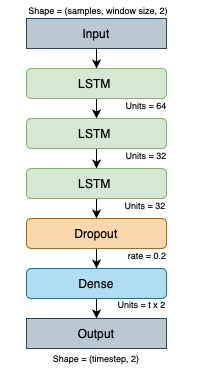
\includegraphics[width=4cm]{pic/ch-Univariate/model-nn.jpg}
    \caption{Illustration of the proposed model}
    \label{fig:nn-model}
\end{figure}

\begin{figure}[t!]
    \centering
    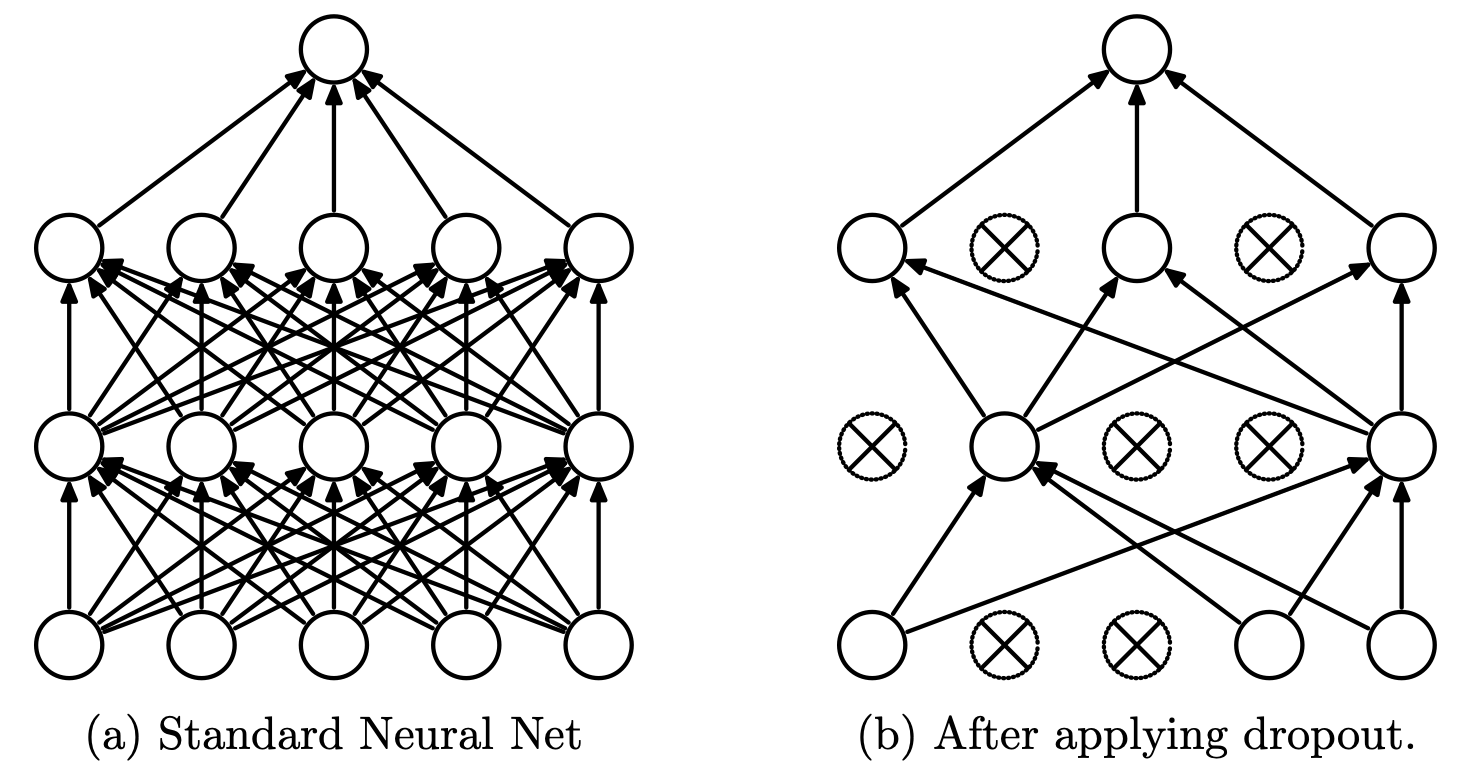
\includegraphics[width=12cm]{pic/ch-Univariate/dropout.png}
    \caption{Dropout Unit Model taken from Srivastava \emph{et al.} Left: A standard neural network of 2 layers. Right: Neural network after some units has been dropped along with its connection.}
    \label{fig:dropout}
\end{figure}

Every layer mentioned above except for Dropout comes with an activation function. Activation functions are function that takes in an argument of input, weight, and overall bias of neuron and decides a specific output value or activation value of the node. Activation function can be either linear or non-linear function depending on the function it represents \cite{nwankpa2018activation}. The linear activation function is amongst the simplest yet limited in functionality due to its linear transformation. Non-linear activation is used to learn more complex functions. In general, the two most widely used non-linear activation are sigmoid and hyperbolic tangent functions. The input to the sigmoid function is transformed into a value between 0 and 1 following an S shape-like curve, which means any value larger than 1 is equal to 1, and a negative value lesser than 0 become 0. Hyperbolic tangent has similar properties as sigmoid with an output value range between -1 to 1. In Keras, default activation function of LSTM is hyperbolic tangent (or \emph{tanh}) and no default function for Dense layer. Generally, we use Rectified Linear Unit (ReLU) function for regression problems for 2 reasons, first ReLU has linear function property for input > 0 which is useful to avoid vanishing gradient problem, and secondly ReLU is a non-linear function.

\subsection{Optimization Algorithm}
The optimization algorithm helps us minimize or maximize loss function (sometimes referred to as the objective function) of the model. There are two major types of optimization algorithms; first-order and second-order optimization. The first-order optimization minimizes the function using \emph{gradient} concerning its function parameters, while the second-order optimization uses \emph{second order derivatives} to find the global minimum of its function. Our model applies a first-order optimization technique as it is more commonly used in deep learning practice. Gradient Descent is the name of the first-order optimization algorithm for finding local minimum by computing the first order derivative of loss function or often referred to as the gradient. The drawbacks of Gradient Descent are mainly being slow in convergence and the algorithm could be stuck in a sub-optimal local minimum. There are 3 variants of Gradient Descent to help resolve its problem; Batch Gradient Descent, Stochastic Gradient Descent (SGD), and Mini-batch Gradient Descent. The difference of each variant mainly in the amount of data being used to compute the gradient of loss function which results in the improvement of computing efficiency and accuracy. However it does not guarantee the algorithm to converge and find the local minimum. Several algorithms have been developed to address such problems by making use of gradient acceleration; including Momentum, Adagrad, Adadelta, RMSProp, Adam, and Nesterov Gradient. Andrej Karpathy, Director of AI at Tesla, analyzed the trend of optimization algorithms used in Arxiv papers from the course of 2012 until 2017 and found out that Adam is used in about 23\% of papers, the highest among other algorithms. RMSProp comes second at 5\%, followed by Adagrad and Adadelta at 4\%. The popularity of Adam and RMSProp in neural network research happens for a reason. We discuss several algorithms related to the development of Adam and RMSProp.

\begin{itemize}
    \item Momentum \cite{qian1999momentum} is an algorithm that helps accelerate the convergence of SGD in the relevant direction using history movement and dampens the oscillation when the gradient changes direction.
    \item Adaptive Gradient or Adagrad \cite{duchi2011adaptive} is an algorithm with an adaptive learning rates which means it computes individual learning rate for different parameters. The learning rate is low for parameters associated with frequently occurring features and set high for a parameter associated with infrequently occurring features \cite{optimizationruder}.
    \item RMSProp is an adaptive learning rate method proposed by Geoffrey Hinton to solve the diminishing learning rate problem in Adagrad.
    \item Adaptive Moment Estimation or Adam \cite{kingma2014adam} can be seen as a combination of Momentum and RMSProp technique resulting in faster convergence with all benefit from RMSProp and Adagrad.
\end{itemize}

Looking at the above discussion, our model will use Adam for the first attempt and switch to RMSProp in the event of a poor result.

\section{Summary}
In this chapter, we gave an overview of the research problem, the methodology we use, and the rationale behind each design choice. An input of the AIS time series dataset was built for two different models of representation, which can be applied to machine learning and recurrent neural network model. We design and implement a baseline model for a problem in hand, which allows us to build a better model in the next chapter.
